\documentclass{beamer}

\mode<presentation>
{
  \usetheme{default}
  \usecolortheme{default}
  \usefonttheme{default}
  \setbeamertemplate{navigation symbols}{}
  \setbeamertemplate{caption}[numbered]
  \setbeamertemplate{footline}[page number]
  \setbeamercolor{frametitle}{fg=white}
  \setbeamercolor{footline}{fg=black}
} 

\usepackage[english]{babel}
\usepackage[utf8x]{inputenc}
\usepackage{tikz}
\usepackage{listings}
\usepackage{courier}
\usepackage{array}
\usepackage{bold-extra}
\usepackage{minted}

\xdefinecolor{darkblue}{rgb}{0.1,0.1,0.7}
\xdefinecolor{darkgreen}{rgb}{0,0.5,0}
\xdefinecolor{darkgrey}{rgb}{0.35,0.35,0.35}
\xdefinecolor{darkorange}{rgb}{0.8,0.5,0}
\xdefinecolor{darkred}{rgb}{0.7,0,0}
\xdefinecolor{dianablue}{rgb}{0.18,0.24,0.31}
\definecolor{commentgreen}{rgb}{0,0.6,0}
\definecolor{stringmauve}{rgb}{0.58,0,0.82}

\lstset{ %
  backgroundcolor=\color{white},      % choose the background color
  basicstyle=\ttfamily\small,         % size of fonts used for the code
  breaklines=true,                    % automatic line breaking only at whitespace
  captionpos=b,                       % sets the caption-position to bottom
  commentstyle=\color{commentgreen},  % comment style
  escapeinside={\%*}{*)},             % if you want to add LaTeX within your code
  keywordstyle=\color{blue},          % keyword style
  stringstyle=\color{stringmauve},    % string literal style
  showstringspaces=false,
  showlines=true
}

\lstdefinelanguage{scala}{
  morekeywords={abstract,case,catch,class,def,%
    do,else,extends,false,final,finally,%
    for,if,implicit,import,match,mixin,%
    new,null,object,override,package,%
    private,protected,requires,return,sealed,%
    super,this,throw,trait,true,try,%
    type,val,var,while,with,yield},
  otherkeywords={=>,<-,<\%,<:,>:,\#,@},
  sensitive=true,
  morecomment=[l]{//},
  morecomment=[n]{/*}{*/},
  morestring=[b]",
  morestring=[b]',
  morestring=[b]"""
}

\title[2017-05-23-ecosystem-dataformats]{Survey of data formats and conversion tools}
\author{Jim Pivarski}
\institute{Princeton University -- DIANA}
\date{May 23, 2017}

\begin{document}

\logo{\pgfputat{\pgfxy(0.11, 8)}{\pgfbox[right,base]{\tikz{\filldraw[fill=dianablue, draw=none] (0 cm, 0 cm) rectangle (50 cm, 1 cm);}}}\pgfputat{\pgfxy(0.11, -0.6)}{\pgfbox[right,base]{\tikz{\filldraw[fill=dianablue, draw=none] (0 cm, 0 cm) rectangle (50 cm, 1 cm);}
\includegraphics[height=0.99 cm]{diana-hep-logo.png}\tikz{\filldraw[fill=dianablue, draw=none] (0 cm, 0 cm) rectangle (4.9 cm, 1 cm);}}}}

\begin{frame}
  \titlepage
\end{frame}

\logo{\pgfputat{\pgfxy(0.11, 8)}{\pgfbox[right,base]{\tikz{\filldraw[fill=dianablue, draw=none] (0 cm, 0 cm) rectangle (50 cm, 1 cm);}
\includegraphics[height=1 cm]{diana-hep-logo.png}}}}

% Uncomment these lines for an automatically generated outline.
%\begin{frame}{Outline}
%  \tableofcontents
%\end{frame}

%%%%%%%%%%%%%%%%%%%%%%%%%%%%%%%%%%%%%%%%%%%%%%%%%%%%%%%

\begin{frame}{The landscape of generic containers}
\vspace{0.25 cm}
``Generic'' file formats are like XML and JSON; can hold anything.

\vspace{0.25 cm}
But we're mostly interested in the binary ones with schemas:

\vspace{0.25 cm}
\mbox{\hspace{-0.75 cm}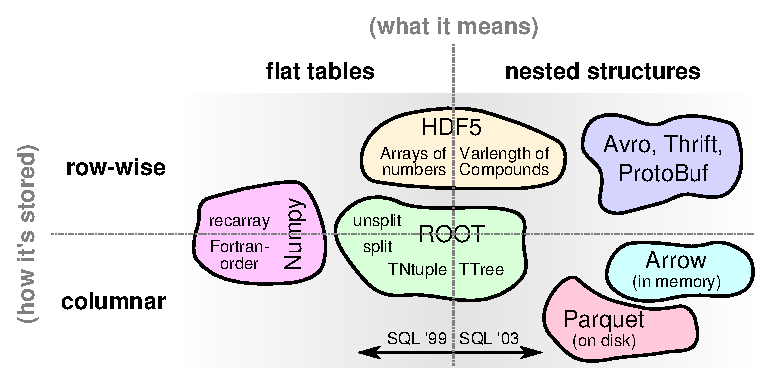
\includegraphics[width=1.15\linewidth]{table-of-formats.pdf}}
\end{frame}

\begin{frame}{The landscape of generic containers}
\vspace{0.25 cm}
\begin{description}\setlength{\itemsep}{0.25 cm}
\item[ROOT:] can do anything with the right settings
\item[HDF5:] stores block-arrays very well, good for flat ntuples; can do e.g.\ lists of particles (``variable-length arrays of compounds''), but not with columnar storage (?)
\item[Numpy:] usually in-memory, but has an efficient file format; only for block-arrays (exceptions not worth using)
\item[Avro et al:] interlingual, binary, deep structures with schemas, row-wise storage is best for streaming and RPC
\item[Parquet:] extension of Avro et al with {\it columnar} storage, intended for databases and fast querying
\item[Arrow:] in-memory extension of the above, intended for zero-copy communication among databases, query servers, analysis frameworks, etc.
\end{description}
\end{frame}

\begin{frame}{Is there a performance penalty?}
\vspace{0.35 cm}
\begin{columns}
\begin{column}{0.55\linewidth}
\begin{itemize}
\item<1-> Formats differ most in how nested structure is represented:
\small

\vspace{0.1 cm}
\textcolor{darkblue}{Avro:} whole records are contiguous

\textcolor{darkblue}{ROOT:} each leaf is contiguous with list sizes in a separate array

\textcolor{darkblue}{Parquet:} each leaf is contiguous with depth in ``repetition levels''

\normalsize
\item<2-> Nevertheless, differences (with gzip/deflate) are only $\sim$20\%. Use-cases may have more variation than choice of format.

\item<3-> Read speed depends greatly on what objects are being created.

\scriptsize
\vspace{0.1 cm}
E.g.\ Avro's C library loads into its custom C objects in 113~sec; Avro's Java library in 8.3~sec! But if you just read through the row-wise data and fill minimalist objects in C, it's 5.4~sec.

\end{itemize}
\end{column}
\uncover<2->{\vrule{}}
\begin{column}{0.5\linewidth}
\begin{onlyenv}<1>
\begin{center}
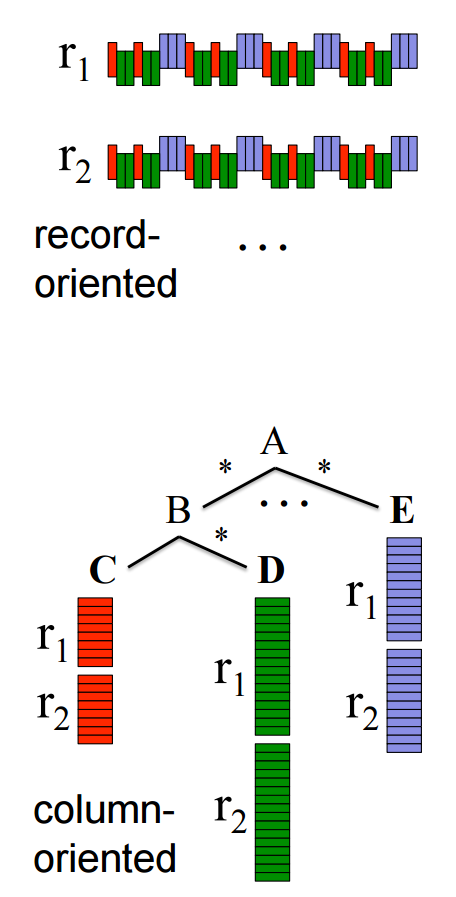
\includegraphics[width=0.5\linewidth]{columnar.png}
\end{center}
\end{onlyenv}
\begin{onlyenv}<2->
\begin{center}
\begin{minipage}{0.9\linewidth}
\scriptsize 47\,407 $t\bar{t}$ Monte Carlo events in {\tt TClonesArrays} or variable-length lists of custom classes.

\vspace{0.1 cm}
ROOT 6.06, Avro 1.8.1, Parquet 1.8.1.
\end{minipage}

\vspace{0.5 cm}
\small
\begin{tabular}{l c c}
format         & MB  & rel. \\\hline
ROOT none      & 399 & 1.96 \\
\textcolor{darkblue}{ROOT gzip 1}    & \textcolor{darkblue}{204} & \textcolor{darkblue}{1.00} \\
ROOT gzip 2    & 208 & 1.02 \\
ROOT gzip 9    & 202 & 0.99 \\\hline
Avro none      & 237 & 1.16 \\
Avro snappy    & 198 & 0.97 \\
\textcolor{darkblue}{Avro deflate}   & \textcolor{darkblue}{180} & \textcolor{darkblue}{0.88} \\
Avro LZMA      & 169 & 0.83 \\\hline
Parquet none   & 210 & 1.03 \\
Parquet snappy & 200 & 0.98 \\
\textcolor{darkblue}{Parquet gzip}   & \textcolor{darkblue}{176} & \textcolor{darkblue}{0.86} \\
\end{tabular}
\end{center}
\end{onlyenv}
\end{column}
\end{columns}
\end{frame}

\begin{frame}{What matters more is how you'll use it}
\vspace{0.5 cm}
\begin{center}
\renewcommand{\arraystretch}{1.3}
\begin{tabular}{r p{0.7\linewidth}}
\textcolor{darkblue}{ROOT} & is the best way to access petabytes of HEP data and use tools developed in HEP \\\hline
\textcolor{darkblue}{HDF5} & is the best way to use tools developed in other sciences, particuarly R, MATLAB \\\hline
\textcolor{darkblue}{Numpy} & is the best way to use the scientific Python ecosystem, particularly recent machine learning software \\\hline
\textcolor{darkblue}{Avro et al} & is the best way to use the Hadoop ecosystem, particularly streaming frameworks \\\hline
\textcolor{darkblue}{Parquet} & is the best way to use database-like tools in the Hadoop ecosystem, such as SparkSQL \\\hline
\textcolor{darkblue}{Arrow} & is in its infancy, but is already a good way to share data between Python (Pandas) DataFrames and R DataFrames \\
\end{tabular}
\end{center}
\end{frame}

\begin{frame}{Conversions: getting from here to there}
\vspace{0.5 cm}
\mbox{\hspace{-0.75 cm}\only<1>{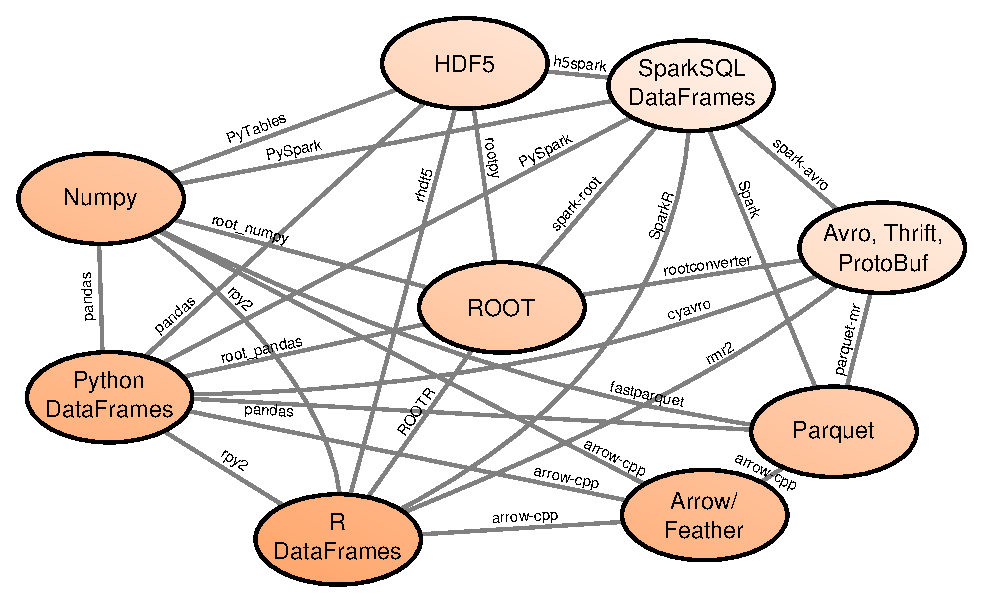
\includegraphics[width=1.15\linewidth]{conversions3.pdf}}\only<2>{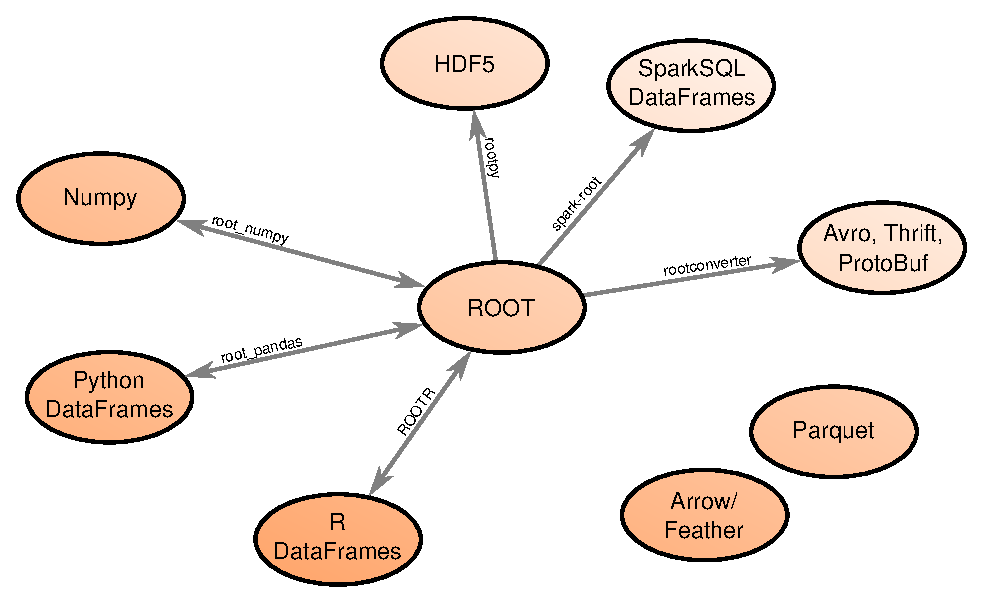
\includegraphics[width=1.15\linewidth]{conversions4.pdf}}\only<3>{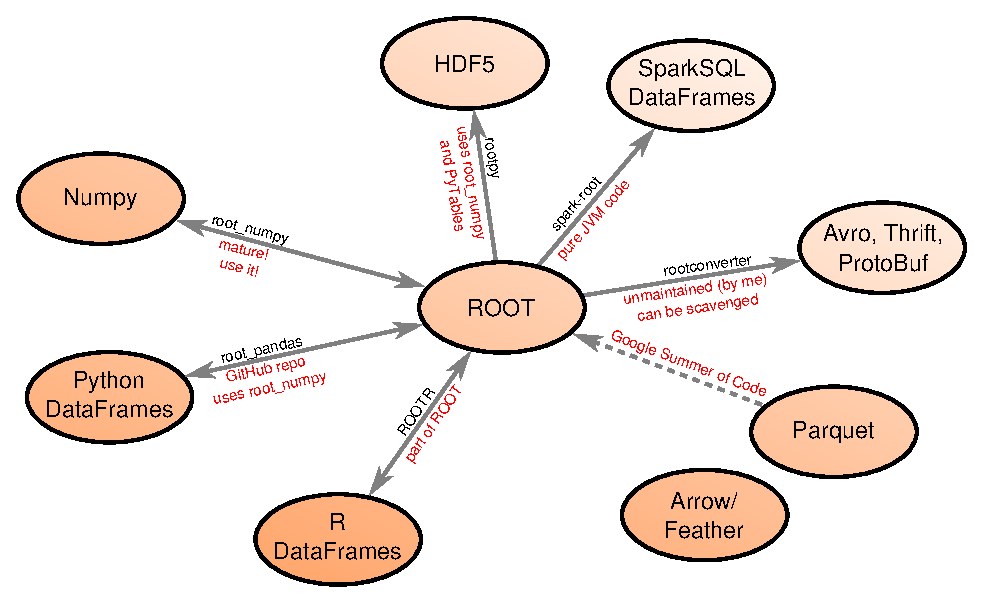
\includegraphics[width=1.15\linewidth]{conversions5.pdf}}}
\end{frame}

\end{document}
